\documentclass{beamer}

\usepackage{colortbl}
\usepackage{tikz}
\usepackage{tikz-qtree}
\usepackage{ifthen}
\usepackage{tikz-uml}
%\usepackage[caption=false]{subfig}
%\usepackage{tabularx}
%\usepackage{color}
\usepackage{amsmath}
\usepackage{listings}
\usepackage{amsfonts}
\usepackage{amsthm}
\usepackage{algpseudocode}
\usepackage{algorithm}

\definecolor{dkgreen}{rgb}{0,0.6,0}
\definecolor{gray}{rgb}{0.5,0.5,0.5}
\definecolor{mauve}{rgb}{0.58,0,0.82}

\lstdefinelanguage{PIL}{
morekeywords={ExecutionOrder, Common, Prover, Verifier, Def, Void, Prime, Z, Int},
otherkeywords={Zmod+, Zmod*},
morecomment=[l]{//},
morecomment=[s]{/*}{*/}
}

\lstdefinelanguage{PSL}{
  morekeywords={Prime, Public, ProverPrivate,
    KnowledgeError, SZKParameter, ProtocolComposition, Homomorphism,
    ChallengeLength, SigmaPhi, Relation, Declarations, Inputs, Properties},
  otherkeywords={Zmod+, Zmod*},
  morecomment=[l]{//}, morecomment=[s]{/*}{*/}
}

\lstdefinelanguage{grammar}{
  keywords={},
  otherkeywords={}
}

\lstdefinelanguage{GEZEL}{
  morekeywords={sfg, dp, always, reg, syg, system, ns, tc, out, in, use, sig, ipblock, iptype},
%  otherkeywords={$display, $hex, $dec, $bin, $cycle},
  morecomment=[l]{//},
}

\lstset{
  basicstyle=\footnotesize,
  commentstyle=\color{dkgreen},
  keywordstyle=\bfseries,
  frame=single,
  breaklines=true,
  breakatwhitespace=false,
}

\usetikzlibrary{backgrounds,calc,shapes,shapes.geometric,shadows,arrows,chains,trees,fit,positioning}

\tikzstyle{language}=[rectangle,draw=black,thin,inner sep=3pt, align=center]

\tikzstyle{compiler}=[rectangle,rounded corners,draw=black,thin,inner
sep=3pt, align=center]

\tikzstyle{added}=[fill=dkgreen]

\usetheme{Warsaw}

\title[Implementation and Evaluation of ZK-PoK]{Implementation and
  Evaluation of Zero Knowledge Proofs of Knowledge}

\author{Boran Car}
\institute{KU Leuven}

\begin{document}

\newcommand{\secret}[1]{\textcolor{red}{#1}}

\begin{frame}
  \titlepage
\end{frame}

\begin{frame}{Outline}
  \tableofcontents[hideothersubsections, pausesections]
\end{frame}

\section{Introduction}
\subsection{Motivation}

\begin{frame}{Current cryptography usage}
  Smart cards, secure web-browsing, \ldots

  \vfill

  \pause

  All involve revealing who the user is
\end{frame}

\begin{frame}{Target applications}
  Targeted applications and developed protocols for
  \begin{itemize}
  \pause \item E-petition
  \pause \item E-voting
  \pause \item E-cash
  \pause \item anonymous credentials (driver's license, \ldots)
  \end{itemize}
\end{frame}

\begin{frame}{Anonymity}
  
  Current electronic methods require the user to log-in. The
  user has no choice but to give away his personal information.

  \vrule

  \pause

  To assure anonymity with voting and petitions, paper methods
  are still used but this is just wasting paper and valuable
  man-hours on counting and processing.
\end{frame}

\subsection{Zero Knowledge Proofs of Knowledge}

\begin{frame}{Zero Knowledge Proofs of Knowledge}
  Allow to prove knowledge of a secret without actually revealing it

  \vfill

  \pause

  We will take an example of anonymous e-petitions. Proving
  that you allowed to sign a petition (of a legal age, from
  a certain town, \ldots)
\end{frame}

\begin{frame}[fragile]{$\Sigma$-protocols}
  Three round protocols

  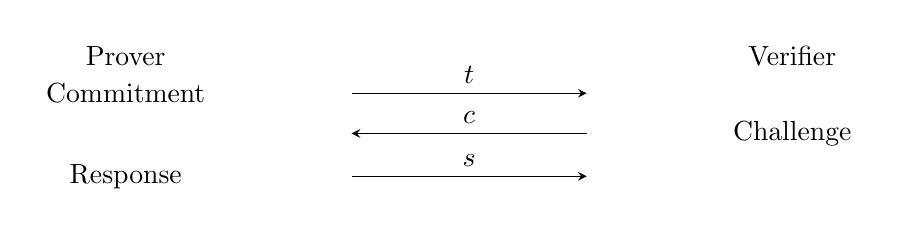
\begin{tikzpicture}[>=stealth]
    \node[matrix,column sep=1.5cm] {
      \node{Prover};                  &                           & &                             & \node{Verifier}; \\
      \node{Commitment};          & \node(commitment_s){}; & & \node(commitment_r){}; & \\
                                      & \node(challenge_r){}; & & \node(challenge_s){}; & \node{Challenge}; \\
      \node{Response}; & \node(response_s){}; & & \node(response_r){}; & \\
    };
    \draw[->] (commitment_s) -- (commitment_r) node[midway, anchor=south]{$t$};
    \draw[<-] (challenge_r) -- (challenge_s) node[midway, anchor=south]{$c$};
    \draw[->] (response_s) -- (response_r) node[midway, anchor=south]{$s$};
  \end{tikzpicture}
\end{frame}

\begin{frame}
  \frametitle{Camenisch-Stadler notation}
  
  A useful notation for representing $\Sigma$-protocols

  \[
  \textrm{ZPK}\left[ (\secret{x}): y = g^{\secret{x}} \right]
  \]

  The example reads: prove knowledge of secret $x$ using the
  homomorphism $y = g^{\secret{x}}$.

  This is Schnorr's Identification Protocol
\end{frame}

\begin{frame}[fragile]{Schnorr's Identification Protocol Flow}
    \begin{tikzpicture}[>=stealth]
      \node[matrix,column sep=1.3cm] {
        \node{Prover};                  &                           & &                             & \node{Verifier}; \\
        \node{$r_1 \in Z_q^+$};                   &                           & &                             &                   \\
        \node{$t_1 = g^{r_1}$};          & \node(prover_round1_s){}; & & \node(verifier_round1_r){}; & \\
                                      & \node(prover_round2_r){}; & & \node(verifier_round1_s){}; & \node{$c \in \{0,1\}^*$}; \\
        \node{$s_1 = r_1 + \secret{x} \cdot c$}; & \node(prover_round2_s){}; & & \node(verifier_round2_r){}; & \\
                                      &                           & &                             & \node{$s_1 \stackrel{?}{\in} Z_q^+$}; \\
                                      &                           & &                             & \node{$t_1 y^c \stackrel{?}{=} g^{s_1}$}; \\
      }; 
      \draw[->] (prover_round1_s) -- (verifier_round1_r) node[midway, anchor=south]{$t_1$};
      \draw[<-] (prover_round2_r) -- (verifier_round1_s) node[midway, anchor=south]{$c$};
      \draw[->] (prover_round2_s) -- (verifier_round2_r) node[midway,anchor=south]{$s_1$};
    \end{tikzpicture}

    The secret $\secret{x}$ is never revealed to the verifier
\end{frame}

\subsection{Original contribution}

\section{Existing frameworks}

\subsection{Domain Specific Languages}

\begin{frame}{Programmers vs. Cryptographers}
  Programmers are not specialists in cryptography and cryptographers
  are not specialists in programming.
\end{frame}

\begin{frame}[fragile]
  \frametitle{C/C++ is dangerous}
  Q: What will the output of the following snippet be?
  \begin{lstlisting}[language=C]
    #include <stdio.h>

    int b(void) { puts("3"); return 3; }
    int c(void) { puts("4"); return 4; }

    int main(void)
    {
      int a = b() + c();
      printf("%d\n", a);

      return 0;
    }
  \end{lstlisting}
  \pause
  A: It can be 3, 4, 7 or 4, 3, 7. The order of evaluation is unspecified.
\end{frame}

\begin{frame}{Domain Specific Languages}
  Q: What is a possible solution for such cases?

  \pause

  A: Languages that are custom designed for a specific application
  (cryptography in our case)
\end{frame}

\subsection{CACE Project Zero Knowledge Compiler}

\begin{frame}{CACE Project ZKC}
  \begin{center}
  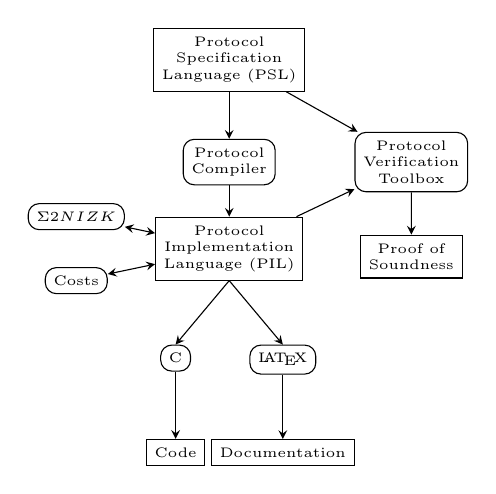
\begin{tikzpicture}[>=stealth,level distance=1.2cm,font=\tiny]
    \tikzstyle{edge from parent}=[draw,->]

    \Tree [.\node[language](psl){Protocol \\ Specification \\ Language (PSL)};
      [.\node[compiler](pc){Protocol \\ Compiler};
        [.\node[language](pil){Protocol \\ Implementation \\ Language (PIL)};
          [.\node[compiler](c){C}; \node[language](code){Code};]
          [.\node[compiler](latex){\LaTeX}; \node[language](doc){Documentation};]
        ]
      ]
    ]

    \node[compiler] (pvt)         [right=of pc,anchor=west]          {Protocol \\ Verification \\ Toolbox}
    child {node[language] {Proof of \\ Soundness}};

    \node[compiler] (sigma) [left=of pil.north west,anchor=center] {$\Sigma 2 N I Z K$};
    \node[compiler] (cost) [left=of pil.south west,anchor=center] {Costs};

    \draw[<->] (sigma) -- (pil);
    \draw[<->] (cost) -- (pil);

    \draw[->] (psl) -- (pvt);
    \draw[->] (pil) -- (pvt);
  \end{tikzpicture}
  \end{center}
\end{frame}

\begin{frame}[fragile]{PSL - Protocol Specification Language}
  Attempts to follow the Camenisch-Stadler notation for specifying
  $\Sigma$ protocols. For example, the Schnorr protocol was given as
  \[
  \textrm{ZPK}\left[ (x): y = g^x \right]
  \]
  and this is specified as:
  \begin{lstlisting}
    SigmaPhi P_1 {
      Homomorphism (phi : Zmod+(q) -> Zmod*(p) : (a) |-> (g^a));
      ChallengeLength := 80;
      Relation ((y) = phi(x));
    }
  \end{lstlisting}
\end{frame}

\begin{frame}{PIL - Protocol Implementation Language}
  The lower-level language. On its own, a well defined Turing complete
  language with support for:
  \begin{itemize}
  \item global constants
  \item global variables
  \item conditionals
  \item loops
  \item functions
  \item predicates
  \item type alias
  \end{itemize}
\end{frame}

\subsection{ZKPDL/Cashlib}

\begin{frame}{ZKPDL/Cashlib}
  Another framework for building ZK-PoK, based on an interpreter
  approach. The language is not Turing complete and the framework is
  limited to non-interactive ZK-PoK.
\end{frame}

\section{Custom framework}

\subsection{Motivation}

\begin{frame}{Custom Framework Motivation}
  Current frameworks are only available for general purpose computers
  while we want to target embedded devices. We also want to allow
  HW-SW co-design exploration.
  \vfill
  \pause
  Some protocols have non-$\Sigma$ sub-protocols, we should also support
  such protocols.
\end{frame}

\subsection{Extensions to CACE}

\begin{frame}{CACE ZKC Extensions}
  \begin{center}
    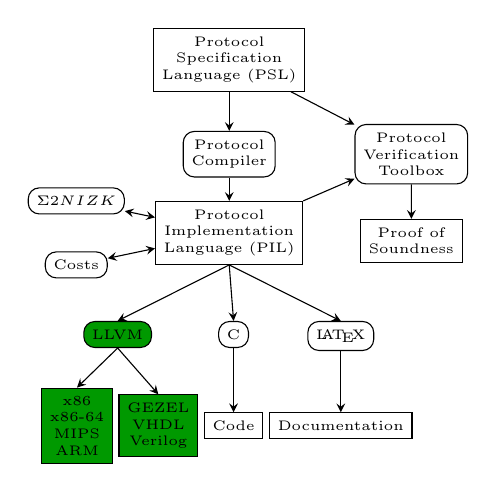
\begin{tikzpicture}[>=stealth,level distance=1.1cm, font=\tiny]
      \tikzstyle{edge from parent}=[draw,->] \tikzset{every leaf
        node/.style={anchor=center}}

      \Tree [.\node[language](psl){Protocol \\ Specification \\ Language (PSL)};
        [.\node[compiler](pc){Protocol \\ Compiler};
          [.\node[language](pil){Protocol \\ Implementation \\ Language (PIL)};
            [.\node[compiler,added](llvm){LLVM};
              \node[language,added](asm){x86 \\ x86-64 \\ MIPS \\ARM};
              \node[language,added](gezel){GEZEL \\ VHDL \\ Verilog};
            ]
            [.\node[compiler](c){C}; \node[language](code){Code};]
            [.\node[compiler](latex){\LaTeX}; \node[language](doc){Documentation};]
          ]
        ]
      ]

      \node[compiler] (pvt)         [right=of pc,anchor=west]          {Protocol \\ Verification \\ Toolbox}
    child {node[language] {Proof of \\ Soundness}};

      \node[compiler] (sigma) [left=of pil.north west,anchor=center] {$\Sigma 2 N I Z K$};
      \node[compiler] (cost) [left=of pil.south west,anchor=center] {Costs};

      \draw[<->] (sigma) -- (pil);
      \draw[<->] (cost) -- (pil);

      \draw[->] (psl) -- (pvt);
      \draw[->] (pil) -- (pvt);
    \end{tikzpicture}
  \end{center}
\end{frame}

\begin{frame}{LLVM}
  A compiler infrastructure framework supporting aggressive optimizations

  \vfill

  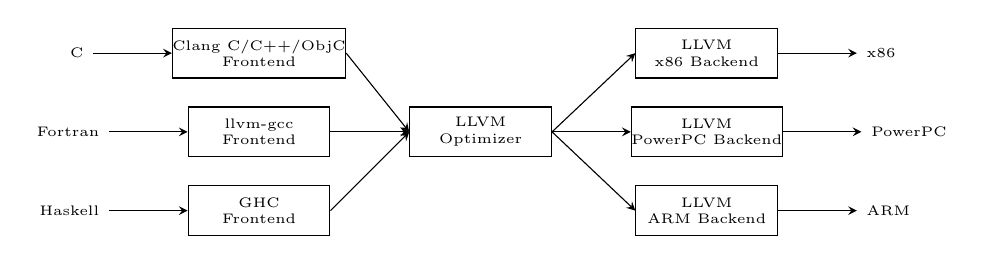
\begin{tikzpicture}[>=stealth]
    \tikzstyle{lang}=[rectangle,draw=black,thin,font=\tiny,inner
    sep=0pt, align=center,minimum width=1.8cm,minimum height=1.8em]

    \tikzstyle{txt}=[font=\tiny]

    \node[lang](llvm_opt){LLVM \\ Optimizer};
    \node[lang](ppc_back)[right=1 cm of llvm_opt]{LLVM \\ PowerPC Backend};
    \node[txt](ppc)[right=of ppc_back]{PowerPC};
    \node[lang](x86_back)[above of=ppc_back]{LLVM \\ x86 Backend};
    \node[txt](x86)[right=of x86_back]{x86};
    \node[lang](arm_back)[below of=ppc_back]{LLVM \\ ARM Backend};
    \node[txt](arm)[right=of arm_back]{ARM};

    \node[lang](gcc_front)[left=1 cm of llvm_opt]{llvm-gcc \\ Frontend};
    \node[txt](fortran)[left=of gcc_front]{Fortran};
    \node[lang](clang_front)[above of=gcc_front]{Clang C/C++/ObjC \\ Frontend};
    \node[txt](c)[left=of clang_front]{C};
    \node[lang](ghc_front)[below of=gcc_front]{GHC \\ Frontend};
    \node[txt](haskell)[left=of ghc_front]{Haskell};

    \draw[->] (clang_front.east) -- (llvm_opt.west);
    \draw[->] (gcc_front.east) -- (llvm_opt.west);
    \draw[->] (ghc_front.east) -- (llvm_opt.west);

    \draw[->] (llvm_opt.east) -- (x86_back.west);
    \draw[->] (llvm_opt.east) -- (ppc_back.west);
    \draw[->] (llvm_opt.east) -- (arm_back.west);

    \draw[->] (x86_back) -- (x86);
    \draw[->] (ppc_back) -- (ppc);
    \draw[->] (arm_back) -- (arm);

    \draw[->] (c) -- (clang_front);
    \draw[->] (fortran) -- (gcc_front);
    \draw[->] (haskell) -- (ghc_front);
  \end{tikzpicture}
\end{frame}

\begin{frame}[fragile]{LLVM IR}
  The intermediate representation which uses variables of SSA form.

  \begin{lstlisting}
    define i80 @Round1(i1024 %_t_1) {
    entry:
      store i1024 %_t_1, i1024* @_t_1
      %calltmp = call i1024 @Random()
      %0 = trunc i1024 %calltmp to i80
      store i80 %0, i80* @_c
      %_c = load i80* @_c
      ret i80 %_c
    }
  \end{lstlisting}

  Resembles a Load-Store RISC architecture ASM language
\end{frame}

\begin{frame}[fragile]{Custom Extensions - PIL Front-end}
    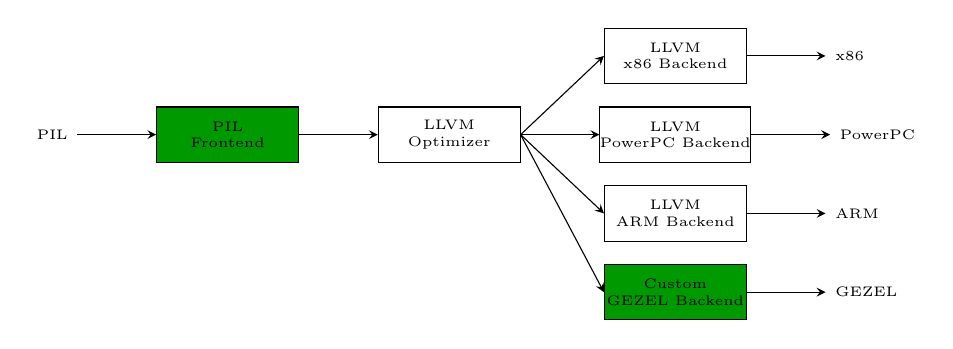
\begin{tikzpicture}[>=stealth, font=\tiny]
      \tikzstyle{lang}=[rectangle,draw=black,thin,inner sep=0pt,
      align=center,minimum width=1.8cm,minimum height=2.0em]

    \tikzstyle{txt}=[]

    \node[lang](llvm_opt){LLVM \\ Optimizer};
    \node[lang](ppc_back)[right=1 cm of llvm_opt]{LLVM \\ PowerPC Backend};
    \node[txt](ppc)[right=of ppc_back]{PowerPC};
    \node[lang](x86_back)[above of=ppc_back]{LLVM \\ x86 Backend};
    \node[txt](x86)[right=of x86_back]{x86};
    \node[lang](arm_back)[below of=ppc_back]{LLVM \\ ARM Backend};
    \node[txt](arm)[right=of arm_back]{ARM};
    \node[lang,added](gezel_back)[below of=arm_back]{Custom \\ GEZEL Backend};
    \node[txt](gezel)[right=of gezel_back]{GEZEL};

    \node[lang,added](pil_front)[left=1 cm of llvm_opt]{PIL \\ Frontend};
    \node[txt](pil)[left=of pil_front]{PIL};

    \draw[->] (pil_front.east) -- (llvm_opt.west);

    \draw[->] (llvm_opt.east) -- (x86_back.west);
    \draw[->] (llvm_opt.east) -- (ppc_back.west);
    \draw[->] (llvm_opt.east) -- (arm_back.west);

    \draw[->] (x86_back) -- (x86);
    \draw[->] (ppc_back) -- (ppc);
    \draw[->] (arm_back) -- (arm);

    \draw[->] (pil) -- (pil_front);

    \draw[->] (llvm_opt.east) -- (gezel_back.west);

    \draw[->] (gezel_back) -- (gezel);
  \end{tikzpicture}

\end{frame}

\subsection{Extensions to PIL}

\begin{frame}[fragile]{Constant expressions}
  Constant expressions

\begin{lstlisting}[language=PIL]
Common (
  Z l_n = 1024;
  Z l_f = 160;
  Z l_phi = 80;
  Z l_H = 160;
  ...
  Prime(l_n) n = 17
) {
}

Smartcard (
  Int(l_f + l_phi + l_H) f;
  ...
\end{lstlisting}
\end{frame}

\begin{frame}{Multiparty protocols}
  Previously only 2 parties were supported: \emph{Prover} and \emph{Verifier}
  
  \vfill

  \begin{center}
  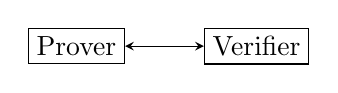
\begin{tikzpicture}[>=stealth]
    \node[language](prover){Prover};

    \node[language](verifier)[right=of prover]{Verifier};

    \draw[<->] (prover) -- (verifier);
  \end{tikzpicture}
  \end{center}

  \vfill

  True multiparty is now supported with arbitrary names

  \vfill

  \begin{center}
  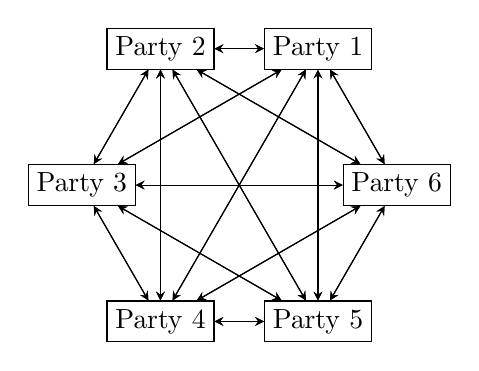
\begin{tikzpicture}[>=stealth]
    \foreach \x in {1,...,6}{
      \node at (\x*360/6:2cm) [language](party_\x){Party \x};
    }

    \foreach \x in {1,...,6}{
      \foreach \y in {1,...,6}{
        \ifthenelse{\not\equal{\x}{\y}}{
          \draw[<->] (party_\x) -- (party_\y);
        }{}
      }
    }
  \end{tikzpicture}
  \end{center}
\end{frame}

\begin{frame}[fragile]{Type inference}
  Deducing the correct type of an expression

  \begin{lstlisting}[language=PIL]
    Zmod*(p) b;
    x := Random(Int(80));
    a := b^x;
  \end{lstlisting}  
\end{frame}

\subsection{PIL Front-end}

\begin{frame}{PIL Front-end}
  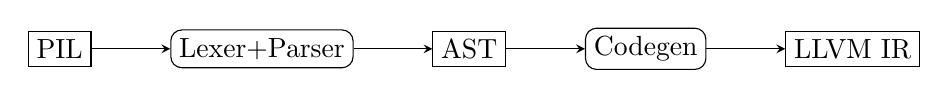
\begin{tikzpicture}[>=stealth]
    \node[language] (pil) {PIL};
    \node[compiler] (lexer_parser) [right=of pil] {Lexer+Parser};
    \node[language] (ast) [right=of lexer_parser] {AST};
    \node[compiler] (codegen) [right=of ast] {Codegen};
    \node[language] (llvm_ir) [right=of codegen] {LLVM IR};

    \draw[->] (pil) -- (lexer_parser);
    \draw[->] (lexer_parser) -- (ast);
    \draw[->] (ast) -- (codegen);
    \draw[->] (codegen) -- (llvm_ir);
  \end{tikzpicture}

  \vfill

  Each party/block is compiled into a separate module with
  the common module linked in

  \vfill

  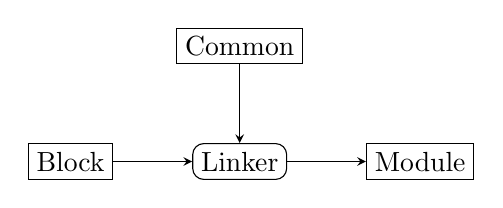
\begin{tikzpicture}[>=stealth]
    \node[language] (block) {Block};
    \node[compiler] (linker) [right=of block] {Linker};
    \node[language] (common) [above=of linker] {Common};
    \node[language] (module) [right=of linker] {Module};

    \draw[->] (block) -- (linker);
    \draw[->] (common) -- (linker);
    \draw[->] (linker) -- (module);
  \end{tikzpicture}
\end{frame}

\begin{frame}[fragile]{How is it generated?}
  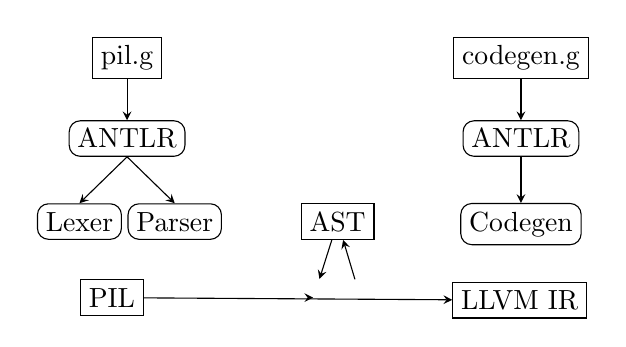
\begin{tikzpicture}[>=stealth]
    \tikzstyle{edge from parent}=[draw,->]

    \node[matrix, column sep=1cm] {
      \Tree[.\node[language](parser_g){pil.g};
        [.\node[compiler](antlr){ANTLR};
          [.\node[compiler](lexer){Lexer};]
          [.\node[compiler](parser){Parser};]
        ]
      ]
      &
      \node[language] (ast) [right=of parser] {AST};
      &
      \Tree[.\node[language](tree_g){codegen.g};
        [.\node[compiler](antlr2){ANTLR};
          [.\node[compiler](walker){Codegen};]
        ]
      ] \\
    };

    \draw[->] (lexer) -- (parser);
    \draw[->] (parser) -- (ast);
    \draw[->] (ast) -- (walker);

    \node[language] (pil) [left=of lexer] {PIL};
    \node[language] (llvm_ir) [right=of walker] {LLVM IR};

    \draw[->] (pil) -- (llvm_ir);
  \end{tikzpicture}
\end{frame}

\begin{frame}[fragile]{Type System}
  \begin{center}
    \begin{tikzpicture}
    \tikzumlset{font=\tiny}

    \umlclass{NumberT}{
      \# width : const uint64\_t
    }{
      \umlvirt{+ getType() : llvm::Type} \\ 
      \umlvirt{+ getBitWidth() : uint64\_t}
    }
    \umlclass[y=-3]{GroupT}{
      \# modulus : const llvm::APInt
    }{
      + getModulus() : llvm::APInt \\
      + getModulusConstant() : llvm::ConstantInt
    }
    \umlinherit{NumberT}{GroupT}
  \end{tikzpicture}
  \end{center}
\end{frame}

\begin{frame}[fragile]{Type Inference}
  \begin{lstlisting}[language=C++]
class NumberT {
  ...
  virtual NumberT *addWithSubFrom(const NumberT *first);
  ...
  virtual NumberT *operator+(const NumberT &other) const {
    return other.addWithSubFrom(this);
  }
};

class GroupT : public NumberT {
  ...
};
\end{lstlisting}
\end{frame}

\subsection{GEZEL Back-end}

\begin{frame}[fragile]{Custom Extensions - GEZEL Back-end}
    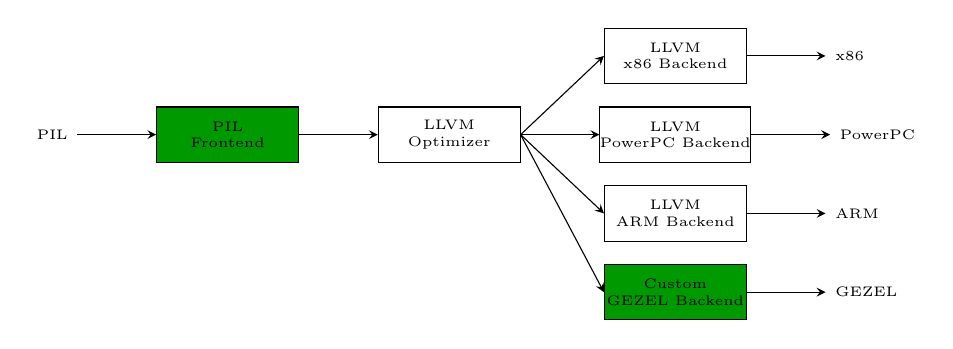
\begin{tikzpicture}[>=stealth, font=\tiny]
      \tikzstyle{lang}=[rectangle,draw=black,thin,inner sep=0pt,
      align=center,minimum width=1.8cm,minimum height=2.0em]

    \tikzstyle{txt}=[]

    \node[lang](llvm_opt){LLVM \\ Optimizer};
    \node[lang](ppc_back)[right=1 cm of llvm_opt]{LLVM \\ PowerPC Backend};
    \node[txt](ppc)[right=of ppc_back]{PowerPC};
    \node[lang](x86_back)[above of=ppc_back]{LLVM \\ x86 Backend};
    \node[txt](x86)[right=of x86_back]{x86};
    \node[lang](arm_back)[below of=ppc_back]{LLVM \\ ARM Backend};
    \node[txt](arm)[right=of arm_back]{ARM};
    \node[lang,added](gezel_back)[below of=arm_back]{Custom \\ GEZEL Backend};
    \node[txt](gezel)[right=of gezel_back]{GEZEL};

    \node[lang,added](pil_front)[left=1 cm of llvm_opt]{PIL \\ Frontend};
    \node[txt](pil)[left=of pil_front]{PIL};

    \draw[->] (pil_front.east) -- (llvm_opt.west);

    \draw[->] (llvm_opt.east) -- (x86_back.west);
    \draw[->] (llvm_opt.east) -- (ppc_back.west);
    \draw[->] (llvm_opt.east) -- (arm_back.west);

    \draw[->] (x86_back) -- (x86);
    \draw[->] (ppc_back) -- (ppc);
    \draw[->] (arm_back) -- (arm);

    \draw[->] (pil) -- (pil_front);

    \draw[->] (llvm_opt.east) -- (gezel_back.west);

    \draw[->] (gezel_back) -- (gezel);
  \end{tikzpicture}

\end{frame}

\begin{frame}{GEZEL Back-end}
  Maximally unrolls the CFG into a single cycle operation. Each
  element of the DFG needs its block counterpart.

  \vfill

  \begin{tabular}{l|r}
    LLVM IR & GEZEL \\
    \hline
    Registers & Signals \\
    Memory & Registers \\
    Multiplication & Multiplier \\
    Exponentiation & Exponentiator
  \end{tabular}
\end{frame}

\begin{frame}{Generated GEZEL Architecture}
    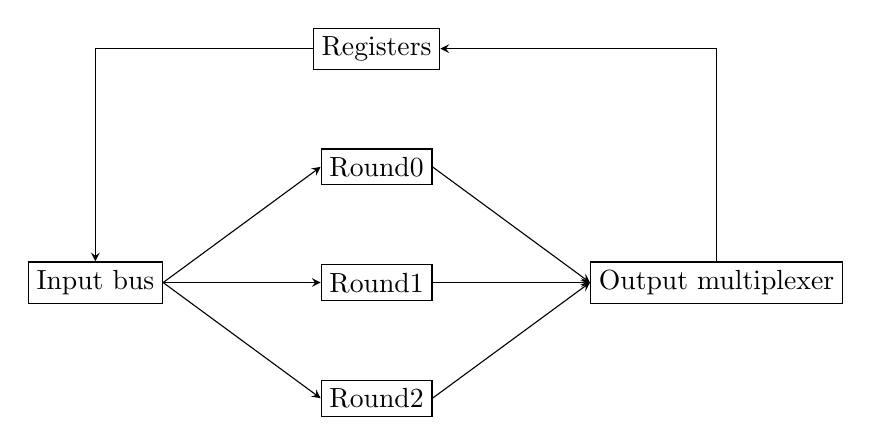
\begin{tikzpicture}[>=stealth]
    \tikzstyle{every node}=[inner sep=0.5cm]
    \node[language](round0){Round0};
    \node[language](round1)[below=of round0]{Round1};
    \node[language](round2)[below=of round1]{Round2};

    \node[language](regs)[above=of round0]{Registers};

    \node[language](mux_in)[left=2cm of round1]{Input bus};

    \node[language](mux_out)[right=2cm of round1]{Output multiplexer};

    \draw[->](round0.east) -- (mux_out.west);
    \draw[->](round1.east) -- (mux_out.west);
    \draw[->](round2.east) -- (mux_out.west);
    \draw[->](mux_in.east) -- (round0.west);
    \draw[->](mux_in.east) -- (round1.west);
    \draw[->](mux_in.east) -- (round2.west);
    \draw[->](regs.west) -- (mux_in.north |- regs.west) -- (mux_in.north);
    \draw[->](mux_out.north) -- (mux_out.north |- regs.east) -- (regs.east);
  \end{tikzpicture}
\end{frame}

\subsection{GEZEL extensions}

\begin{frame}[fragile]{Terminal communication}
  Allows GEZEL to communicate to the ``outside'' world

  \begin{lstlisting}[language=GEZEL]
    ipblock my_term(in tx    : ns(1024);
                    out rx   : ns(1024);
                    in sr    : ns(2);
                    out done : ns(1)) {
      iptype "transceiver";
    }
  \end{lstlisting}

  Also allowed for cross-validation with the code generated by CACE ZKC
\end{frame}

\begin{frame}[fragile]{Modular exponentiation}
  A change was made to GEZEL to allow modular exponentiation
  operations

  \begin{lstlisting}
    y = g ** x % p;
  \end{lstlisting}

  so that a modular exponentiator block can be instantiated and used
\end{frame}

\subsection{Example}

\begin{frame}{Schnorr's Identification Protocol Example}
  CACE Project Zero Knowledge Compiler converts input PSL into PIL

  \vfill

  \pause

  Our framework converts PIL into LLVM IR

  \vfill

  \pause

  then LLVM IR to GEZEL
\end{frame}

\section{Direct Anonymous Attestation}

\begin{frame}{Direct Anonymous Attestation}
  A 3 party protocol

  \vrule

  \hfil 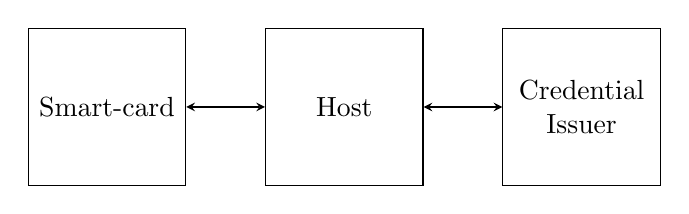
\begin{tikzpicture}[>=stealth]
    \tikzstyle{every node}=[minimum size=2cm]

    \node[language](host){Host};
    \node[language](smartcard)[left=of host]{Smart-card};
    \node[language](issuer)[right=of host]{Credential \\ Issuer};

    \draw[<->] (smartcard) -- (host);
    \draw[<->] (host) -- (issuer);
  \end{tikzpicture}
\end{frame}

\begin{frame}{Direct Anonymous Attestation Phases}
  The protocol consists of 2 phases
  \begin{enumerate}
  \pause \item Join Protocol - establishing of a credential
  \pause \item Sign Protocol - signing using the credential
  \end{enumerate}

  \pause

  The Sign protocol is a Zero Knowledge Proof of Knowledge
\end{frame}

\subsection{Join protocol}

\begin{frame}[fragile]{Join Protocol}
  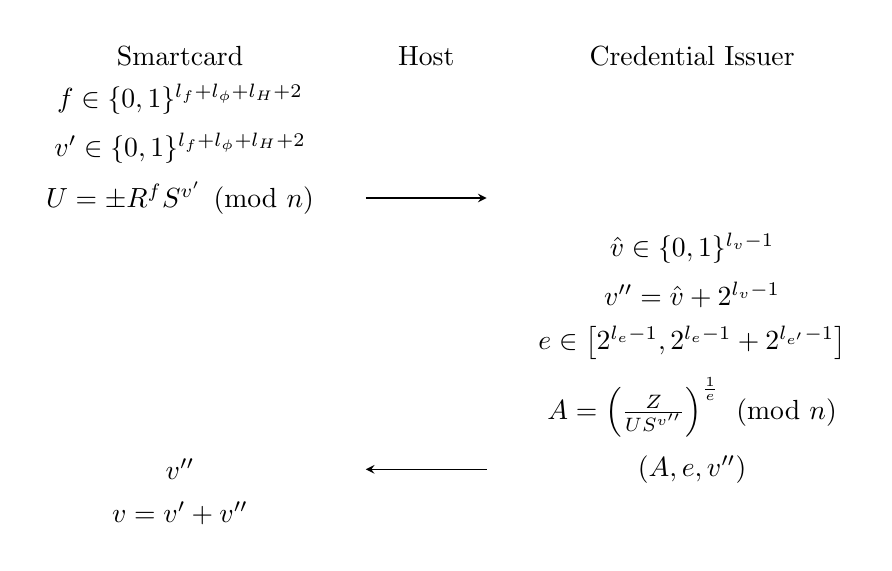
\begin{tikzpicture}[>=stealth]
    \node[matrix,column sep=0.3cm] {
      \node{Smartcard};                       &                           & \node{Host}; &                             & \node{Credential Issuer}; \\
      \node{$f \in \{0,1\}^{l_f+l_\phi+l_H+2}$};   &                           &              &                             &                   \\
      \node{$v' \in \{0,1\}^{l_f+l_\phi+l_H+2}$};  &                           &              &                             &                   \\
      \node{$U = \pm R^f S^{v'} \pmod{n}$};     & \node(scard_round1_s){};  &              & \node(cred_round1_r){};     & \\
                                               &                           &              &                             & \node{$\hat{v} \in \{0,1\}^{l_v-1}$}; \\
                                               &                           &              &                             & \node{$v'' = \hat{v} + 2^{l_v-1}$}; \\
                                               &                           &              &                             & \node{$e \in \left[ 2^{l_e-1}, 2^{l_e-1} + 2^{l_{e'}-1} \right]$}; \\
                                               &                           &              &                             & \node{$A = \left( \frac{Z}{U S^{v''}} \right)^{\frac{1}{e}} \pmod{n}$}; \\
      \node{$v''$};                            & \node(scard_round2_r){};  &              & \node(cred_round1_s){};     & \node{$(A, e, v'')$};\\
      \node{$v = v' + v''$};                   &                           &              &                             & \\
    };
    \draw[->] (scard_round1_s) -- (cred_round1_r);
    \draw[<-] (scard_round2_r) -- (cred_round1_s);
  \end{tikzpicture}
\end{frame}

\subsection{Implementation in PIL}

\begin{frame}[fragile]{Smartcard PIL}
\begin{lstlisting}[language=PIL]
Smartcard () {
  Int(l_f + l_phi + l_H+2) f;
  Int(l_n + l_phi) v_1;
  Int(l_v) v;

  Def (Zmod*(n) U): Round0(Void) {
    f := Random(Int(l_f + l_phi + l_H + 2));
  
    v_1 := Random(Int(l_f + l_phi + l_H + 2));

    U := R^f * S^v_1;
  }

  Def (Void): Round1(Int(l_v-1) v_2) {
    v := v_1 + v_2;
  }
}
\end{lstlisting}
\end{frame}

\begin{frame}[fragile]{Host PIL}
\begin{lstlisting}[language=PIL]
Host (

) {
  Zmod*(n) A;
  Int(l_e) e;
  
  Def (Zmod*(n) U_o): Round0(Zmod*(n) U_i) {
    U_o := U_i;
  }

  Def (Int(l_v-1) v_2_o): Round1(A; e; Int(l_v-1) v_2_i) {
    v_2_o := v_2_i;
  }
}
\end{lstlisting}
\end{frame}

\begin{frame}[fragile]{Credential Issuer PIL}
\begin{lstlisting}[language=PIL]
Credential (

) {
  Def (Zmod*(n) A; Int(l_e) e; Int(l_v-1) v_2): Round0(Zmod*(n) U) {
    v := Random(Int(l_v-1));
    v_2 := v + 2^(l_v-1);
    e := Random([2^(l_e-1), 2^(l_e-1) + 2^(l_e_1-1)]);
    A := (_Z * (U * S^v_2)^(-1))^(e^(-1));
  }
}
\end{lstlisting}
\end{frame}

\section{Conclusions}

\begin{frame}{Conclusions}
  Where does this framework currently stand?

  What can it offer?
\end{frame}

\begin{frame}{Easy to specify protocols}
  The framework makes it easy to specify a protocol in a domain
  specific language by just transcribing the protocol flow.
\end{frame}

\begin{frame}{HW-SW co-design exploration}
  The framework allows for HW-SW co-design exploration by allowing
  2 poles (the pure HW and the pure SW). Lower and upper bounds
  can be derived.
\end{frame}

\begin{frame}{Terminal communication}
  Terminal communication is introduced into both the custom and the
  CACE framework. This allows for cross-validation with developed
  embedded devices.
\end{frame}

\section{Future Work}

\begin{frame}{Future Work}
  Where can this framework go?

  What other work can be derived from it?
\end{frame}

\begin{frame}{Automated HW-SW Co-design Trade-offs}
  Controlled CFG-DFG balancing via a user provided parameter. This
  allows ``sweeping'' of the HW-SW spectrum.
\end{frame}

\begin{frame}{Pseudo Virtual Machines for Tiny Micro-controllers}
  Realized via function calls in C. Since C is an industry standard
  compiler, this extends the possible target architectures.
\end{frame}

\begin{frame}{Extending LLVM IR with Group Types}
  Currently the framework tracks types and backs them with
  available LLVM IR types.
\end{frame}

\begin{frame}{Common Low-level Language for the CACE Project}
  Each of the CACE Projects uses its own low-level language. There
  should be a common infrastructure at the lowest level. LLVM IR
  offers great possibilities thanks to the plethora of architectures
  LLVM supports.
\end{frame}

\begin{frame}{Thank you for your time}
  Questions?
\end{frame}

\end{document}

%%% Local Variables: 
%%% TeX-PDF-mode: t
%%% TeX-master: t
%%% End: 
